\chapter{Virtualização}
\label{cap:virtualizacao}

O conceito virtualização surgiu na década de 60, onde o usuário muitas vezes necessitava de um ambiente individual, 
com suas próprias aplicações e totalmente isolado dos demais usuários. Esse foi um dos principais motivos para a criação das máquinas 
virtuais, que na época eram conhecidas como \ac{VM}. As \acp{VM} apresentaram uma forte expansão com o sistema operacional \textit{370}, que foi 
desenvolvido pela \textit{IBM}, e foi um dos principais sistemas comerciais com suporte à virtualização da época. Esse sistema operacional 
era executado em \textit{mainframes}, que eram grandes servidores capazes de processar um grande volume de informações \cite{laureano2008}. 

Na década de 80 houve uma redução no uso da virtualização devido a popularização do \ac{PC}. Na época era mais vantajoso disponibilizar 
um \ac{PC} para cada usuário do que investir em \textit{mainframes}. Devido à crescente melhora na performance do \ac{PC} e
ao surgimento da linguagem \textit{Java}, no início da década de 90, a tecnologia de virtualização retornou com o conceito de virtualização
de aplicação \cite{laureano2008}.

A virtualização foi definida nos anos 60 e 70 como uma camada entre o \textit{hardware} e o sistema operacional que possibilitava a 
divisão e a proteção dos recursos físicos. Porém, atualmente ela abrange outros conceitos, como por exemplo a \ac{JVM}, que não virtualiza
um \textit{hardware}. De fato, a \ac{JVM} permite que uma aplicação convidada execute em diferentes tipos de sistemas operacionais.

Atualmente, define-se virtualização como uma camada de \textit{software} que utiliza os serviços fornecidos por uma determinada interface de 
sistema para criar outra interface de mesmo nível. Assim, a virtualização permite a comunicação entre interfaces distintas, de forma que uma 
aplicação desenvolvida para uma plataforma \textit{X} possa também executar em uma plataforma \textit{Y} \cite{laureano2008}.

Como mencionado, a virtualização permite a comunicação entre diferentes interfaces, sendo que existem diferentes tipos de interfaces
nos sistemas de computação \cite{maziero2013}:
\begin{itemize}
 \item Conjunto de instruções ou \ac{ISA}: é a interface básica, que fica entre o \textit{software} e o \textit{hardware}, e é composta por 
 instruções de código de máquina. Essa interface é dividida em dois grupos:
 \begin{itemize}
  \item Instruções de usuário ou \textit{User \ac{ISA}}: são instruções disponíveis à aplicações de usuários. Essas instruções executam em 
  modo usuário, sendo que neste modo existem restrições que procuram garantir um controle e segurança no acesso aos recursos de \textit{hardware}. 
  Instruções de usuário são instruções não privilegiadas, ou seja, são instruções que podem ser executadas sem interferir em outras tarefas, 
  porque elas não acessam recursos compartilhados. Este grupo de interface contém, por exemplo, instruções de operações aritméticas e instruções 
  de ponto flutuante \cite{buyya2013};
  %Caso uma instrução privilegiada for executada no modo usuário, ela manifesta-se através de uma interrupção e será devidamente tratada;
  \item Instruções de sistema ou \textit{System \ac{ISA}}: essas instruções geralmente são disponibilizadas para o núcleo do sistema operacional. 
  Elas são instruções privilegiadas, ou seja, são instruções que acessam recursos compartilhados. Essas instruções são executadas em modo 
  supervisor (ou modo \textit{kernel}), que permite realizar operações sensíveis\footnote[1]{Operações sensíveis são instruções que podem alterar o 
  estado do processador.} no \textit{hardware} \cite{buyya2013}. Como exemplo de instruções de sistema pode-se citar as instruções que alteram 
  o estado dos registradores do processador; % entrada e saída (E/S)
 \end{itemize}
 \item Chamadas de sistema ou \textit{syscalls}: são operações oferecidas pelo núcleo do sistema operacional para as aplicações dos usuários.
 Essas operações permitem um acesso controlado aos dispositivos, a memória e ao processador. 
 As instruções privilegiadas não podem ser executadas no modo usuário, por isso, as aplicações de usuários utilizam chamadas de sistemas em seu 
 lugar, e então o sistema operacional determina se essas operações poderão comprometer ou não a integridade do sistema \cite{marinescu2013}.
 Um exemplo de chamada de sistema é uma operação de escrita em disco rígido ou qualquer operação de entrada e saída feita por aplicações de usuários.
\end{itemize}

A Figura \ref{fig:interfaces_isa} mostra as diferentes interfaces entre aplicações de usuários, bibliotecas, núcleo do sistema operacional e o 
\textit{hardware}.

\begin{figure}[h!]
 \centering
 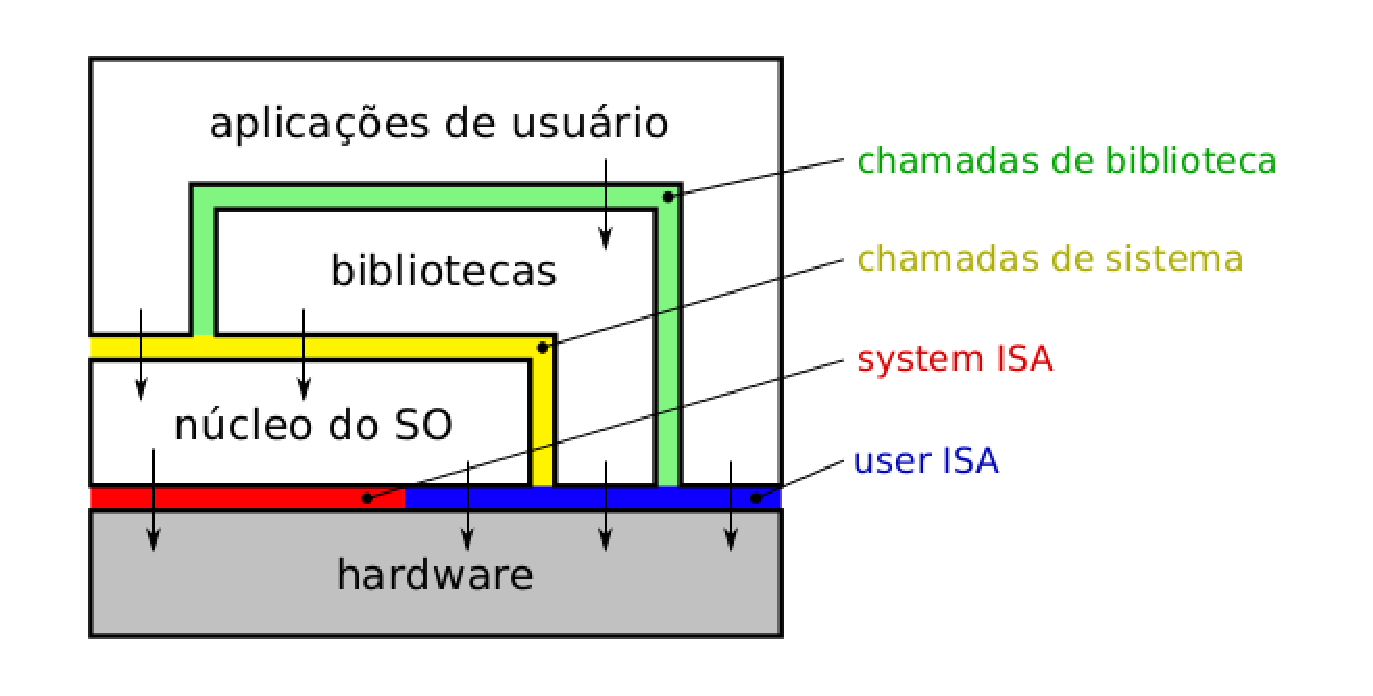
\includegraphics[width=300px]{img/interfaces_isa.eps}
 \caption{Interfaces de sistemas de computação.}
 \label{fig:interfaces_isa}
 Fonte: \citet{maziero2013}
\end{figure}

Máquinas virtuais podem ser divididas em dois grupos principais, que são: as máquinas virtuais de aplicação (Seção \ref{section:virtaplicacao}), 
e máquinas virtuais de sistema (Seção \ref{section:virtsistema}). As máquinas virtuais de aplicação fazem a virtualização de uma aplicação e 
suportam apenas uma aplicação, ou seja, elas provêm um ambiente que permite a execução de uma aplicação convidada. Um exemplo de máquina 
virtual de aplicação é a \ac{JVM}. Já uma máquina virtual de sistema suporta um sistema operacional convidado, com suas aplicações executando 
sobre ele. Uma máquina virtual executando sobre o hipervisor \ac{KVM} \cite{kvm} é um exemplo de máquina virtual de aplicação \cite{laureano2008}.

Na Figura \ref{fig:vms_tipos} (a) tem-se o modelo de máquina virtual de aplicação, onde uma \ac{JVM}, juntamente com aplicações, está executando 
sobre um sistema operacional hospedeiro. A Figura \ref{fig:vms_tipos} (b) apresenta uma máquina virtual de sistema, que possui dois sistemas 
operacionais executando sobre um único \textit{hardware} por meio do hipervisor.

\begin{figure}[h!]
 \centering
 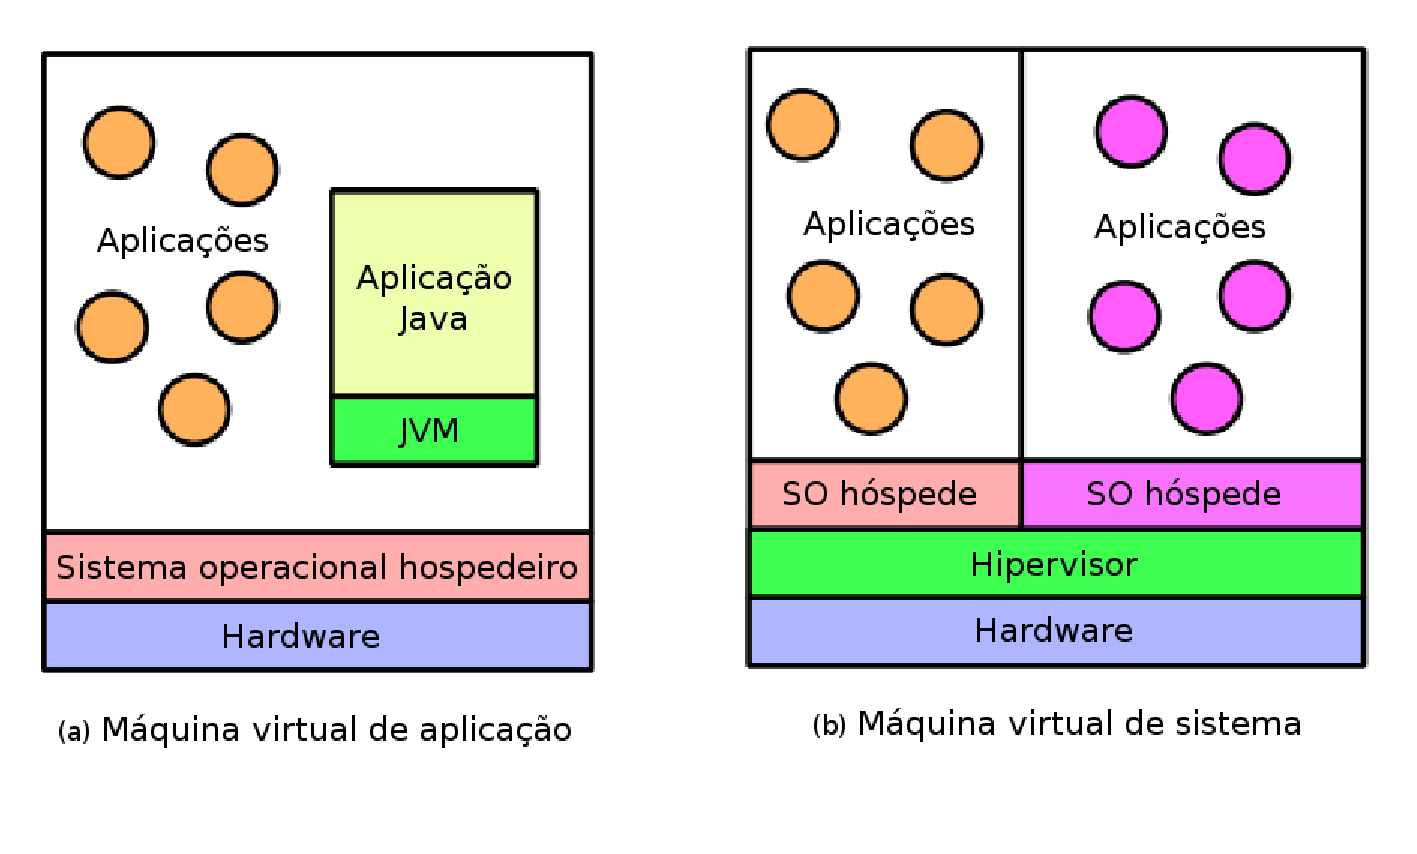
\includegraphics[width=420px]{img/vms_tipos.eps}
 \caption{Máquinas virtuais de aplicação e de sistema.}
 \label{fig:vms_tipos}
 Fonte: \citet{laureano2008}
\end{figure}

\section{Máquinas virtuais de aplicação}
\label{section:virtaplicacao}

As máquinas virtuais de aplicação, também chamadas de máquinas virtuais de processos, são responsáveis por prover um ambiente que permite 
a execução de uma aplicação convidada, sendo que esta aplicação possui um conjunto de instruções, ou de chamadas de sistema, diferentes da 
arquitetura do sistema hospedeiro. Neste caso, quando temos uma chamada de sistema ou instruções de máquina, será necessário uma 
tradução dessas interfaces, que será feita pela camada de virtualização. Os dois principais tipos de máquinas virtuais de aplicação são:

\begin{itemize}
 \item Máquinas virtuais de linguagem de alto nível: esse tipo de máquina virtual foi criado levando em consideração uma linguagem de 
 programação e o seu compilador. Neste caso, o código compilado gera um código intermediário que não pode ser executado em uma arquitetura real, 
 mas pode ser executado em uma máquina virtual. Sendo assim, para cada arquitetura ou sistema operacional deverá existir uma máquina virtual que
 permita a execução da aplicação. Como exemplo deste tipo de máquina virtual pode-se citar a máquina virtual Java (\ac{JVM})
 e a \textit{Microsoft Common Language Infrastructure}, que é a base da plataforma \textit{.NET} \cite{carissimi2008};
 \item Emulação do sistema operacional: nesse caso é feito um mapeamento entre as chamadas de sistema que são utilizadas pela aplicação 
 e as chamadas de sistema operacional hospedeiro. A virtualização de aplicação pode ser encontrada em ferramentas que emulam uma aplicação que foi
 desenvolvida para uma plataforma em uma outra plataforma. Como exemplo, pode-se citar o \textit{Wine} \cite{wine}, que permite executar 
 aplicações \textit{Windows} em plataformas \textit{Linux}.
\end{itemize}

%Na virtualização de aplicação também existem máquinas virtuais que utilizam as mesmas interfaces \ac{ISA} do computador real,
%com isso uma grande parte das instruções podem ser executadas diretamente, com exceção de instruções privilegiadas, que serão devidamente
%tratadas. Alguns tipos de máquinas virtuais de aplicação que utilizam as interfaces do sistema real são:

%\begin{itemize}
% \item Sistemas operacionais multitarefas: sistemas operacionais que suportam simultaneamente mais de um usuário também podem ser
% vistos como máquinas virtuais. Em um sistema multitarefa cada processo possui um ``processador virtual'' (devido a rápida troca de 
% contextos do processador real), uma ``memória virtual'' (memória alocada para o processo) e outros recursos que podem ser acessados
% através de chamadas de sistema;
% \item Tradutores dinâmicos: esses tradutores analisam e otimizam o código de máquina para torná-lo mais eficiente. Essa otimização 
% pode ser feita durante a carga do processo na memória ou durante a execução das instruções. Pode-se citar como exemplo o \ac{JIT} 
% \textit{Bytecode compiler};
% \item Depuradores de memória: são sistemas de depuração de memória que detectam erros decorrentes do uso incorreto da memória.
% Um exemplo de depurador é o sistema \textit{Valgrind}, que utiliza uma máquina virtual para efetuar essa depuração.
%\end{itemize}

\section{Máquinas virtuais de sistema}
\label{section:virtsistema}

As máquinas virtuais de sistema, também chamadas de hipervisor ou \ac{VMM}, são uma camada de \textit{software} que possibilita
que múltiplos sistemas operacionais convidados executem sobre um mesmo computador físico, ou seja, o hipervisor provê uma interface
\ac{ISA} virtual, que pode ou não ser igual a interface real, e virtualiza outros componentes de \textit{hardware}, para que cada máquina
virtual convidada possa ter seus próprios recursos. Para tanto, a virtualização de sistema utiliza abstrações em sua arquitetura. 
Por exemplo, ela transforma um disco rígido físico em dois discos virtuais menores, sendo que esses discos virtuais são arquivos armazenados no 
disco físico \cite{smithenair2005}.
%Sabendo que arquivos são uma abstração em um disco rígido físico, pode-se dizer que virtualização não é apenas uma camada de abstração 
% do \textit{hardware}, ela faz a reprodução do \textit{hardware} \cite{smithenair2005}.

Nesse modelo, o ambiente de virtualização de sistema é composto basicamente por três componentes (Figura \ref{fig:virtcomponentes}):
\begin{itemize}
 \item Máquina real: também chamada de hospedeiro, que é o \textit{hardware} onde o sistema de virtualização irá executar;
 \item Camada de virtualização: é conhecida como hipervisor ou também chamada de \ac{VMM}. Essa camada tem como função criar interfaces 
 virtuais para a comunicação da máquina virtual com a máquina real;
 \item Máquina virtual: também conhecida como sistema convidado, sendo executado sobre a camada de virtualização. Geralmente, tem-se
 várias máquinas virtuais executando simultaneamente sobre esta camada.
\end{itemize}

\begin{figure}[h!]
 \centering
 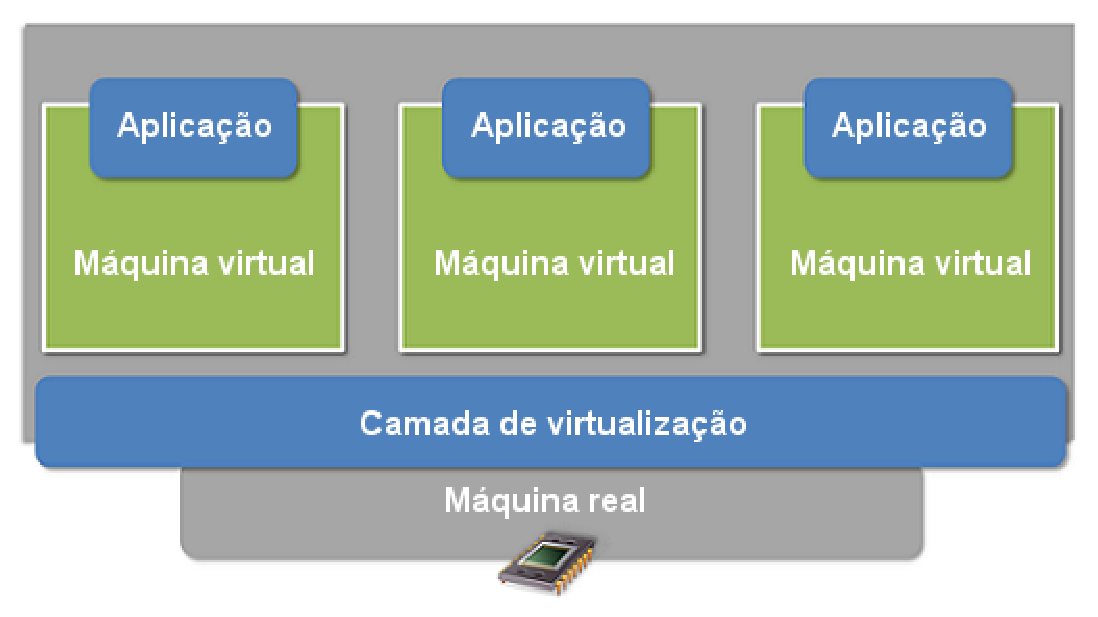
\includegraphics[width=300px]{img/virtcomponentes.eps}
 \caption{Componentes da virtualização.}
 \label{fig:virtcomponentes}
 Fonte: \citet{andrade2011}
\end{figure}

\subsection{Arquiteturas de máquinas virtuais de sistema}
\label{section:virtarquit}

Existem basicamente duas arquiteturas de hipervisor de sistema, que são apresentadas na Figura \ref{fig:vms_arquiteturas} \cite{maziero2013}:

\begin{itemize}
 \item Hipervisores nativos: esse hipervisor executa diretamente sobre o \textit{hardware}, ou seja, sem um sistema operacional
 hospedeiro. Neste caso, o hipervisor nativo faz a multiplexação dos recursos do \textit{hardware} (memória, disco rígido, interface de rede, 
 entre outros) e disponibiliza esses recursos para as máquinas virtuais. Alguns exemplos de sistemas que utilizam essa arquitetura de hipervisor 
 são o \textit{IBM 370} \cite{ibm370}, o \textit{Xen} \cite{xen} e o \textit{VMware ESXi} \cite{vmwareesxi};
 \item Hipervisores convidados: esse tipo de hipervisor executa sobre um sistema operacional hospedeiro e utiliza os recursos desse sistema 
 para gerar recursos para as máquinas virtuais. Normalmente esse tipo de arquitetura suporta apenas um sistema operacional convidado para cada 
 hipervisor. Exemplos de \textit{softwares} que possuem esse tipo de arquitetura são o \textit{VirtualBox} \cite{virtualbox}, 
 o \textit{VMware Player} \cite{vmwareplayer} e o \textit{QEmu} \cite{qemu}.
\end{itemize}

\begin{figure}[h!]
 \centering
 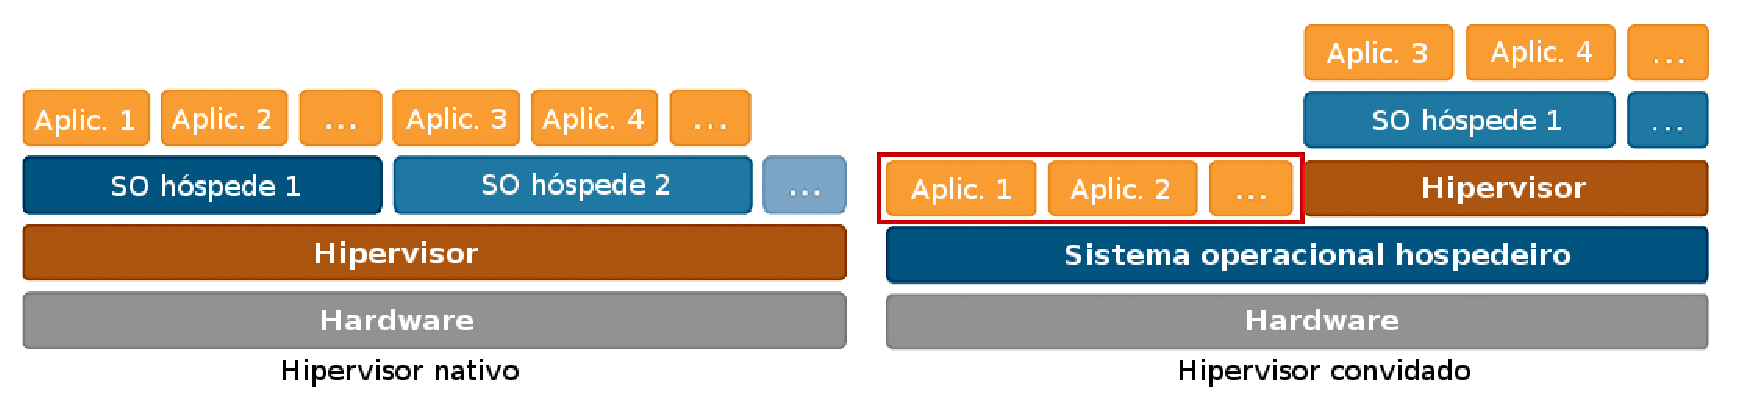
\includegraphics[width=430px]{img/vms_arquiteturas.eps}
 \caption{Arquiteturas de máquinas virtuais de sistema.}
 \label{fig:vms_arquiteturas}
 Fonte: \citet{macedo2016}
\end{figure}

Os hipervisores convidados são mais flexíveis que os nativos, pois podem ser facilmente instalados ou removidos de um sistema operacional já 
instalado. Por outro lado, os hipervisores nativos possuem melhor desempenho pois acessam o \textit{hardware} de forma direta.

%\subsection{Níveis de virtualização}
%\label{section:virtniv}
%\begin{itemize}
% \item Virtualização de recursos: neste tipo de virtualização os recursos como memória e disco, além das instruções 
% privilegiadas (\textit{system \ac{ISA}}) são virtualizadas. Somente a interface \ac{ISA} de usuário é utilizada diretamente, 
% por isso o desempenho do sistema convidado é mais próximo a um sistema executando diretamente sobre um \textit{hardware}. O 
% \textit{VirtualBox} e o \textit{VirtualPC da Microsoft} são exemplos de virtualização de recursos;
% \item Virtualização completa: na virtualização completa todas interfaces são virtualizadas. Sendo assim o hipervisor fornece uma
% interface distinta ao sistema operacional convidado. Esse tipo de virtualização possui um eficiência menor, por outro lado ele
% permite executar sistemas operacionais em plataformas distintas a qual foram projetadas inicialmente. Por exemplo, o 
% \textit{MS Virtual PC for MAC}, que permite executar o sistema \textit{Windows} sobre plataforma de \textit{hardware} \textit{PowerPC}.
%\end{itemize}

%Tendo essas classificações, pode-se combiná-las para se obter quatro maneiras diferentes de implementar virtualização. Na Figura 
%\ref{fig:vms_classificacao} tem-se essas combinações com seus respectivos exemplos.

%\begin{figure}[vms_classificacao]
% \centering
% 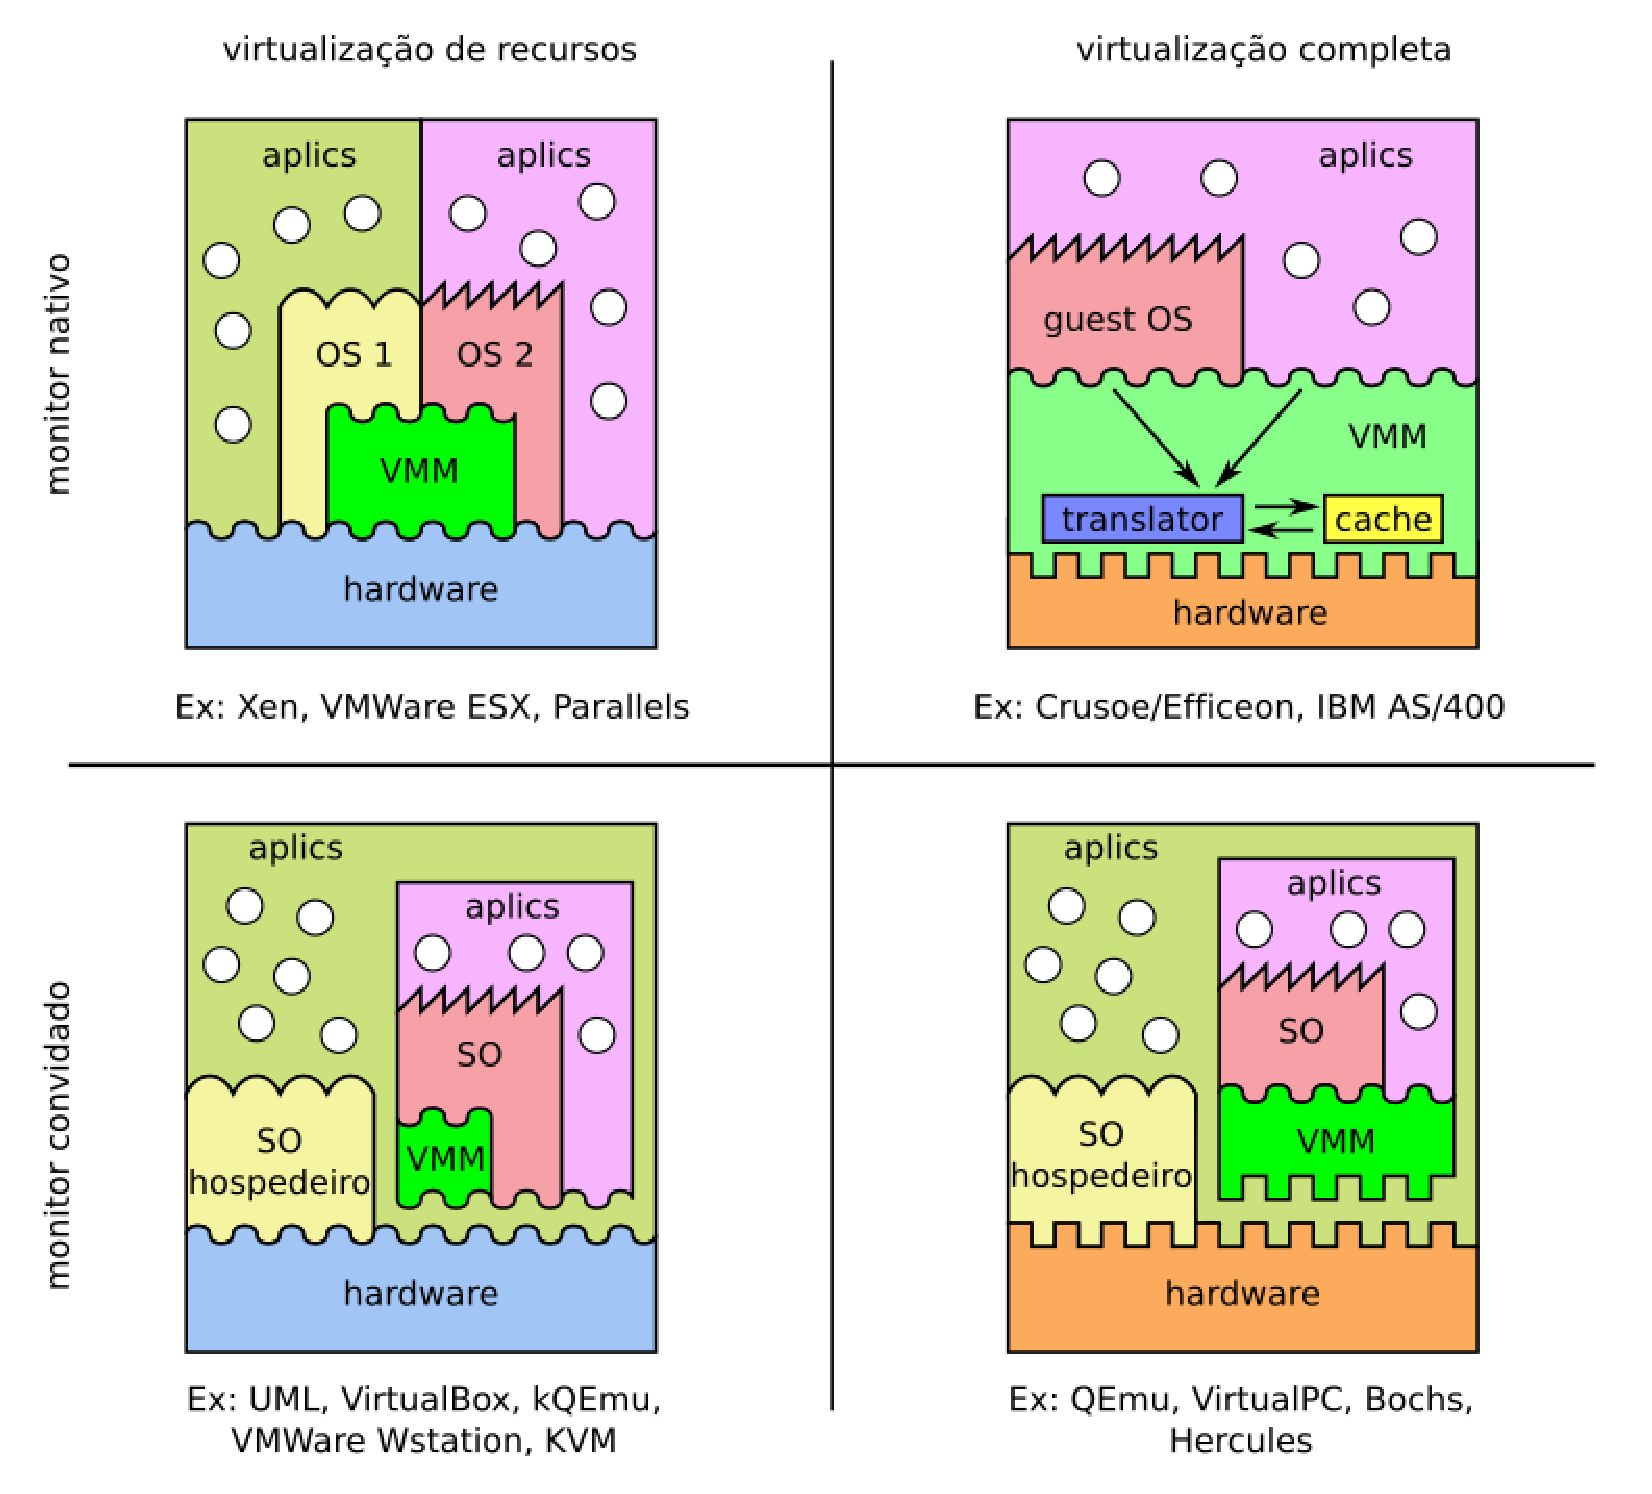
\includegraphics[width=400px]{img/vms_classificacao.eps}
% \caption{Classificação de máquinas virtuais de sistema.}
% \label{fig:vms_classificacao}
% Fonte: \citet{laureano2008}
%\end{figure}

\newpage
\subsection{Implementações de máquinas virtuais de sistema}
\label{section:virtestrat}

As máquinas virtuais de sistema podem ser implementadas usando diferentes estratégias. Atualmente as estratégias mais utilizadas
são a virtualização total e a paravirtualização (Figura \ref{fig:vms_implementacao}):

\begin{figure}[h!]
 \centering
 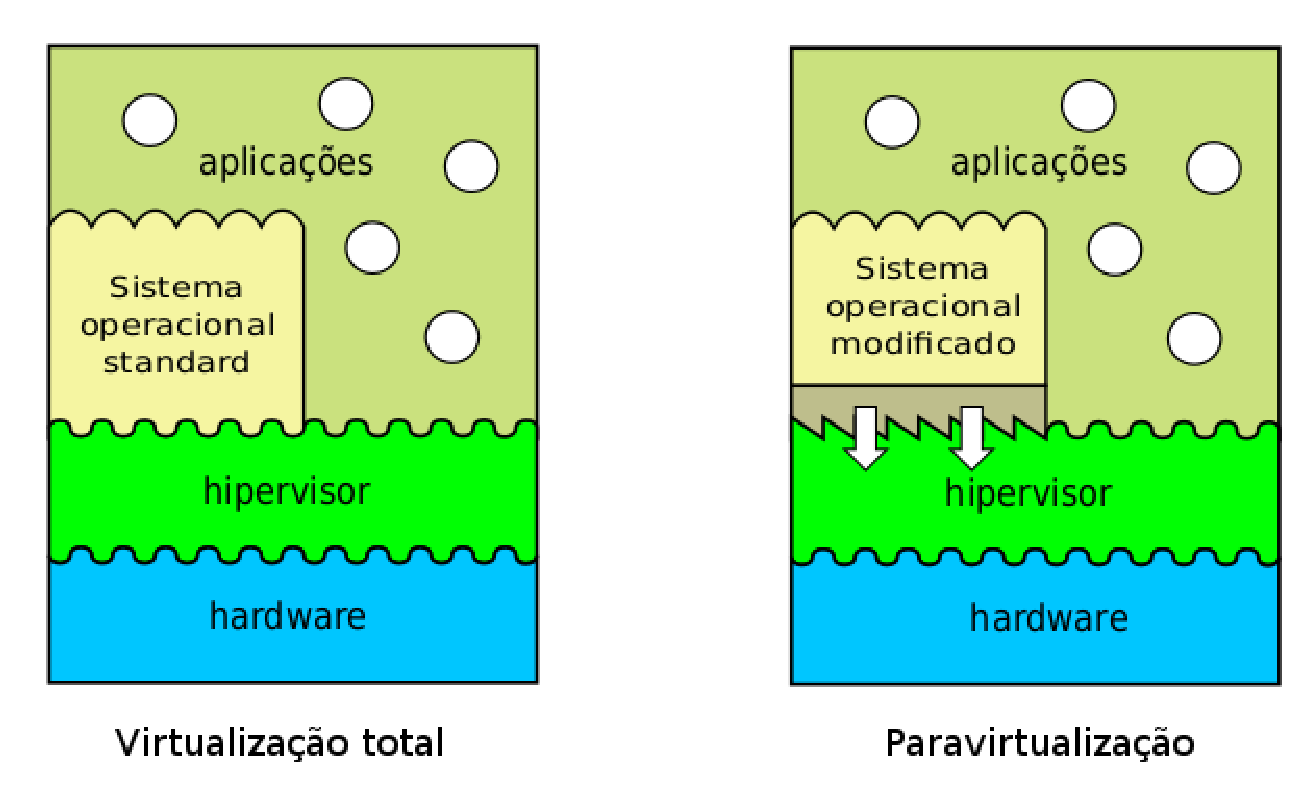
\includegraphics[width=330px]{img/vms_implementacao.eps}
 \caption{Implementações de máquinas virtuais de sistema.}
 \label{fig:vms_implementacao}
 Fonte: \citet{maziero2013}
\end{figure}

\begin{itemize}
 \item Virtualização total: nesta estratégia todas as interfaces de acesso ao \textit{hardware} são virtualizadas. Desta forma, possibilita-se 
 que os sistemas operacionais convidados executem como se estivessem diretamente sobre o \textit{hardware}. Na virtualização total o conjunto de 
 instruções do processador é acessível somente ao hipervisor, sendo que essa estratégia utiliza tradução dinâmica\footnote[1]{A tradução dinâmica 
 analisa e reorganiza as instruções de um sistema convidado para melhorar o desempenho da execução. Além disso, a tradução dinâmica converte as 
 instruções do sistema convidado para o sistema real.} para executar as instruções do sistema convidado. A grande vantagem dessa estratégia é a 
 possibilidade de um sistema convidado ser executado sem a necessidade de ser modificado. Porém, essa estratégia possui um desempenho inferior 
 devido ao fato do hipervisor intermediar todas as chamadas de sistemas e operações do sistema convidado. Um exemplo de ferramenta que utiliza 
 a virtualização total é o \textit{QEmu} \cite{qemu};
 \item Paravirtualização: nesta estratégia a interface entre o hipervisor e o sistema operacional convidado é modificado para se obter uma 
 maior eficiência. Destaca-se que essa estratégia de implementação utiliza uma arquitetura de hipervisor nativo. 
 As modificações na interface de sistema (\textit{system \ac{ISA}}) exigem que o sistema operacional convidado seja adaptado para o hipervisor, 
 para possibilitar a execução sobre a plataforma virtual. Para essa adaptação, o hipervisor disponibiliza uma \ac{API}, para que os 
 sistemas convidados possam acessar o \ac{ISA} de sistema. Contudo, a interface de usuário é mantida, assim, as aplicações do sistema convidado 
 não precisam ser modificadas \cite{maziero2013}.
\end{itemize}

A paravirtualização possui um desempenho superior se comparada a virtualização total, pois acessa alguns recursos de forma direta, sendo que 
o hipervisor é responsável somente por impedir que o sistema convidado execute operações indevidas. Como exemplo pode-se citar o controle de
acesso à memória feito pelo hipervisor. Na virtualização total o hipervisor reserva um espaço para cada sistema convidado, que por sua vez, 
acessa a memória como se fosse uma memória física, ou seja, inicia o seu endereçamento na posição zero. Sendo assim, cada vez que o sistema 
convidado acessar a memória, o hipervisor precisará converter os endereços do sistema convidado para os endereços reais de memória. Já na 
paravirtualização, o hipervisor informa ao sistema convidado a área de memória que ele poderá utilizar, assim, não sendo necessário nenhuma 
conversão de endereços \cite{maziero2013}.

Apesar de apresentar um desempenho inferior, a virtualização total possui uma maior portabilidade, ou seja, permite que sistemas operacionais 
executem como convidados sem a necessidade de serem modificados. Desta forma, qualquer sistema operacional pode ser instalado em um ambiente 
de virtualização total. Além disso, essa técnica permite virtualizar um sistema operacional já instalado apenas copiando o conteúdo de seu disco 
rígido, sem a necessidade de reinstalar esse sistema operacional e reconfigurar todas as aplicações.

\section{Vantagens das máquinas virtuais}
\label{section:virtvantag}

De modo geral, a principal vantagem das máquinas virtuais de aplicação é a possibilidade de executar uma mesma aplicação em diversos sistemas 
operacionais sem a necessidade de recompilar a mesma. Já para máquinas virtuais de sistema, destaca-se a possibilidade de executar mais de um 
sistema operacional sobre um mesmo \textit{hardware}. Nas próximas seções serão descritas as principais utilizações e vantagens da virtualização 
de \textit{desktops} e de servidores.

\subsection{Virtualização de Desktop}
\label{section:virtdesk}

A portabilidade é uma das grandes vantagens da virtualização, que também pode ser aplicada em \textit{desktops}. Pode-se citar como exemplo, 
o desenvolvimento de \textit{software} para diversos sistemas operacionais sem a necessidade de aquisição de um computador físico para a instalação
de cada sistema operacional. Assim, a virtualização de \textit{desktops} pode ser utilizada em ambientes de desenvolvimento, pois possibilitam 
a execução de múltiplas plataformas de desenvolvimento sem comprometer o sistema operacional original \cite{carissimi2008}. Um exemplo é o 
\textit{VMware Workstation}, que possibilita a virtualização em \acp{PC} para fins de desenvolvimento de \textit{software} \cite{vmware2016}.

Em empresas pode-se ainda utilizar a virtualização de \textit{desktops}, através da configuração de terminais remotos nos computadores e um 
servidor para centralizar as máquinas virtuais. Com isso torna-se mais simples a manutenção dos \textit{desktops}, além disso, estes necessitam 
de um \textit{hardware} de menor valor, uma vez que esses executarão apenas um terminal remoto. Por fim, essa técnica possibilita uma maior 
segurança dos dados, pois os dados serão armazenados em um local seguro, como por exemplo, um \textit{data center}. Exemplos desse tipo de 
virtualização são o \textit{Xen Desktop} \cite{xendesktop} e o \textit{VMware Horizon View} \cite{vmwareview}.
%Em empresas pode-se utilizar virtualização de \textit{desktops} para reduzir a subutilização dos \textit{desktops}, que pode ser feito através da
%colaboração com projetos científicos de \textit{clusters} de computadores virtuais \cite{carissimi2008}. %exemplo seti@home

Para usuários de computadores em geral a virtualização também é interessante, uma vez que esses podem necessitar de um \textit{software} que não
está disponível para a plataforma utilizada. Deste modo, a virtualização possibilita executar diferentes sistemas operacionais no computador do 
usuário. Por exemplo, para um usuário de sistema operacional \textit{MacOS} é comum a necessidade de executar aplicações que não existem para a 
sua plataforma, sendo assim esse pode utilizar uma máquina virtual para executar essas aplicações.

Pode-se também encontrar virtualização de \textit{desktops} em laboratórios de ensino, devido a necessidade de executar diferentes sistemas 
operacionais para determinadas disciplinas. Isso é necessário quando pretende-se configurar e executar aplicações para fim de experimentos ou
aprendizagem, com isso, essas ações não afetarão o sistema hospedeiro. A grande vantagem da utilização de máquinas virtuais nesse tipo de 
ambiente é a facilidade na manutenção, pois as máquinas virtuais podem ser restauradas de forma simples.

\subsection{Virtualização de servidores}
\label{section:virtserv}

Em muitos casos as empresas utilizam serviços distribuídos entre diferentes servidores físicos, como por exemplo, servidores de \textit{e-mail}, 
hospedagens de sites e banco de dados. Essa estrutura faz com que alguns recursos fiquem ociosos, pois em muitos casos esses serviços necessitam 
de uma quantidade de recursos inferior ao que o servidor físico oferece. Por exemplo, um serviço de transmissão de \textit{streaming} de áudio 
utiliza pouco acesso ao disco rígido, porém utiliza um poder de processamento e memória RAM maior. Portanto, uma das grandes vantagens da 
virtualização é um melhor aproveitamento dos recursos. De fato, alocando vários serviços em um único servidor físico tem-se um melhor 
aproveitamento do \textit{hardware} \cite{moreira2006} e, consequentemente, tem-se uma redução nos custos de administração e manutenção 
dos servidores físicos.

% A Figura \ref{fig:virtualizacao_servidores}, o servidor localizado à esquerda, apresenta um servidor tradicional com seu sistema operacional 
% (na cor azul) e suas aplicações (na cor laranja). E o servidor à direita é um servidor de virtualização, que possui o hipervisor 
% (na cor azul claro) e suas máquinas virtuais acima do hipervisor.
% \begin{figure}[h!]
%  \centering
%  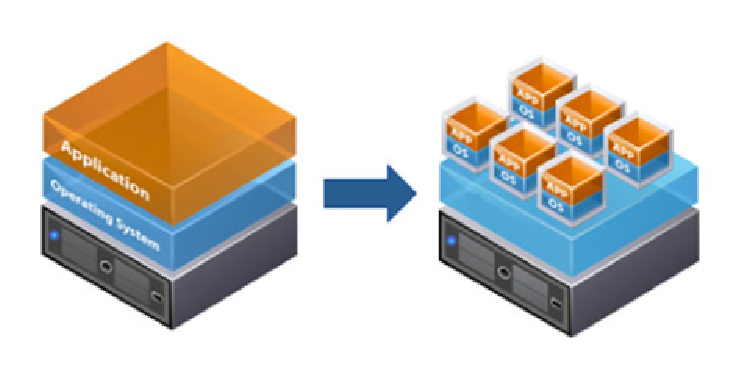
\includegraphics[width=250px]{img/virtualizacao_servidores.eps}
%  \caption{Servidor tradicional e servidor de virtualização.}
%  \label{fig:virtualizacao_servidores}
%  Fonte: \citet{interspire2016}
% \end{figure}

Em um ambiente heterogêneo pode-se também utilizar virtualização, pois ela permite a instalação de diversos sistemas operacionais em um 
único servidor. Esse tipo de virtualização favorece a implementação do conceito ``um servidor por serviço'', que consiste em ter um servidor 
para cada serviço. Além disso, tem-se o isolamento de serviços, ou seja, caso ocorra uma falha de segurança em um serviço, essa falha não 
comprometerá todo o sistema, uma vez que cada serviço estará executando em seu próprio sistema operacional \cite{carissimi2008}.

Outra motivação para a utilização de virtualização em servidores consiste na redução de custos com energia elétrica e equipe que faz a manutenção. 
Essa redução de custos pode ser obtida através da implantação de servidores mais robustos para substituir dezenas de servidores comuns. 
Além disso, pode-se obter uma redução nos custos com refrigeração, uma vez que essa estrutura proporciona uma redução no número de servidores
e do espaço físico necessário para esses.

Por fim, existe uma técnica chamada \textit{live migration}, ou migração em tempo real. Essa técnica possibilita que uma máquina virtual, 
que está executando em um servidor físico, seja transferida, através da rede, para outro servidor sem ser reiniciada. Nesse processo a máquina 
virtual fica no estado suspenso (por um período curto de tempo) até que o servidor de destino receba os dados necessários para continuar 
a execução da máquina virtual \cite{silva2009}. Essa técnica possibilita a utilização de redundância de \textit{software}.

\section{Considerações finais}

Neste capítulo foi apresentado um breve histórico da virtualização e os dois principais grupos de máquinas virtuais existentes, que são: máquinas 
virtuais de aplicação e máquinas virtuais de sistema. Também foram apresentadas as vantagens e as estratégias de implementação de máquinas virtuais, 
dando ênfase para as máquinas virtuais de sistema, uma vez que essas serão utilizadas no desenvolvimento deste trabalho. De fato, essas serão 
utilizadas para a implementação da redundância de \textit{software}. No próximo capítulo será feito o levantamento e análise dos serviços 
fornecidos pela empresa que está sendo estudada neste trabalho. Posteriormente, serão apresentados os serviços que são considerados críticos 
e a proposta de solução de alta disponibilidade.
